\chapter{使用した技術}
%rosについてもっと深堀する
%例:パッケージの作り方,ノードの作り方,パブリッシャーとはなにか,サブスクライバーとはなにか
%ROSのパブリッシャーとサブスクライバーの作り方,mROS 2の作り方embeddedRTPSについても話せるとよい
%C++とpythonの違いを述べる.本実装ではなぜC++を選択したのかを書く
%ついでにサービスとアクションについても述べる
%messageの中身についても語りたい.後で説明が楽になる
\label{sec:usage}
\section{ROS 2}
ROS 2は,ROSの後継であり,ROS 2はROS 1と比べて,分散型のロボットシステムに対応している.
ROS 1では,主にUDPを使用したメッセージ型の通信を行っていたが,ROS 2では,DDS(Data Distribution Service)と呼ばれる通信ミドルウェアを採用しており,RTPS(Real Time Publish Subscribe)プロトコルを用いた
メッセージ型通信を行っている.これによって,個々のロボットが独立して動作するだけでなく,複数のロボットが協調して動作することが可能になった.
\subsection{パブリッシャーとサブスクライバー}
ROSでは,パブリッシャー(Publisher)とサブスクライバー(Subscriber)という2つのノードと呼ばれる間でメッセージをやり取りする仕組みがある.
ノードはパブリッシャーにもサブスクライバーにもプログラム次第で変化できるため,ユーザがオリジナルのノードを作成することができる.
パブリッシャーは,トピックと呼ばれるメッセージの種類を決め,そのトピックに対してメッセージを送信する.
サブスクライバーは,パブリッシャーが送信したメッセージの型を設定して受け取る.
例えば,ROS 2ではパブリッシャーはrclcpp::Publisherクラスを,サブスクライバーはrclcpp::Subscriptionクラスを使用して実装する.
このようにROSは独自の通信機能を用いることによって,一つ一つのノードがそれぞれ役割を持ち,一つになってシステムを構築することができる.
\subsection{ノードの作り方とパッケージ}
ROS 2においてノードを作成する場所は決まっており,一般的にはros2_ワーキングスペース(ws)というディレクトリを作った後,その中にsrcというディレクトリを作成し,その中にノードを作成する.
srcディレクトリを作成した後,ros2_wsディレクトリでcolcon buildというコマンドを実行することで,ros2_wsの中でノードを作成することがきる.
ROS 2の場合,ノードの集まりのことをパッケージと呼ぶ.
パッケージはros2 pkg createというコマンドを実行することで作成することができ,srcディレクトリの直下で実行することで,パッケージを作成することができる.
パッケージを作成する前にそのパッケージの中で使用する言語を決める必要がある.
ROS 2はC++とPythonの2つの言語をサポートしており,ユーザーの好みに合わせて変更できる.
\subsection{オーバーレイとアンダーレイ}
また,ROS 2には重要な概念にアンダーレイとオーバーレイがある.
アンダーレイは,完成されたパッケージをインストールするワークスペースであり,安定した環境をオーバーレイに提供するためにある.
オーバーレイは,ユーザー自身で作成したパッケージを扱うワークスペースであり,先ほどのros2_wsはオーバーレイにあたる.
ROS 2ではユーザーが作るノードやパッケージをオーバーレイに作成し,必要に応じてアンダーレイのパッケージを参照して使用するのが一般的である.
このオーバーレイ上でユーザはcolcon buildを実行し,パッケージをビルドする.
ユーザーはパッケージをビルドした後,すぐに実行することができない.ROS 2ではsourceコマンドを用いてオーバーレイ環境を読み込むことでアンダーレイがオーバーレイより優先されることなく,開発することができる.
ROS 2においてオーバーレイとアンダーレイは,複雑化するロボットシステムに柔軟性と拡張性をもたらす概念であることがわかる.
ROS 2のデバック方法として様々なコマンドが用意されており,ros2 topic listというコマンドを実行することで,現在実行されているトピックの一覧を表示することができる.
また,現在実行されているノードを視覚的に確認できるようにrqt_graphと呼ばれるものが用意されている.開発者はrqt_graphを用いて,目に見えないROS 2のノード間の通信を確認することができる.
こうしたアンダーレイ機能の充実によって,ROS 2はROS 1よりも柔軟性と拡張性を持つことができた.
\subsection{ROS 2が対応しているDDS}
ROS 2にはデフォルトでFastRTPSというDDSが実装されている.
DDSとは,OMG(Object Management Group)が定めたデータ交換のための仕様である.これによって分散型ネットワークでも効率的に通信が可能になっている.
FastRTPSのほかにも,RTI Connext DDSやeProsima Micro XRCE-DDSというDDSがROS 2に対応している.
Ubuntu22.04のROS 2 humbleでは,FastRTPSはもちろんのこと,デフォルトでEcripse Cyclone DDS,Gurum DDS,RTI Connext DDSがインストールできる[https://docs.ros.org/en/humble/Installation/DDS-Implementations.html#ubuntu-linux-source-install].
\subsection{サービスとアクション}

\section{mROS 2-POSIX}
\begin{figure}[ht]
    \centering
    \begin{minipage}{.48\textwidth}
        \centering
        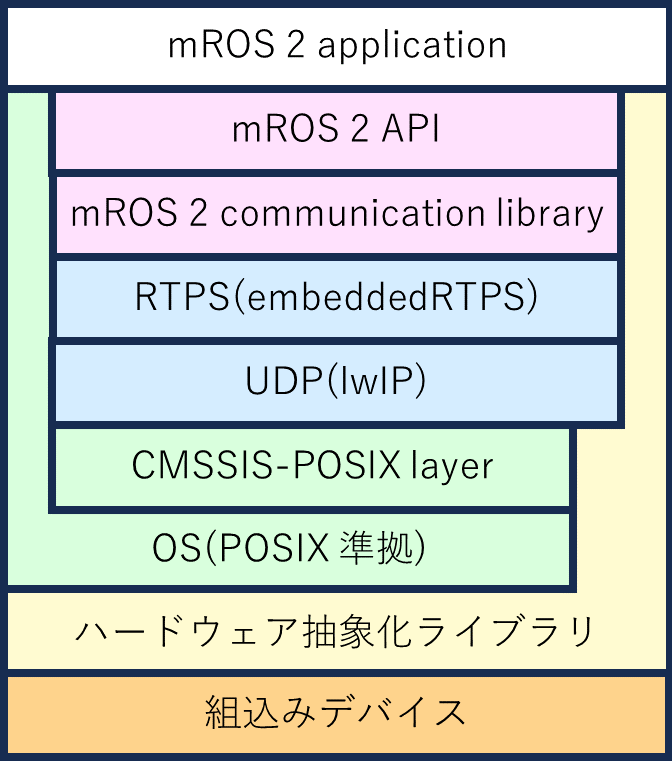
\includegraphics[width=0.9\linewidth]{images/fig1_mros2posix_a.png}
        \caption{mROS 2-POSIXの内部構成}
        \label{fig:subfig_a}
    \end{minipage}
    \hfill
    \begin{minipage}{.48\textwidth}
        \centering
        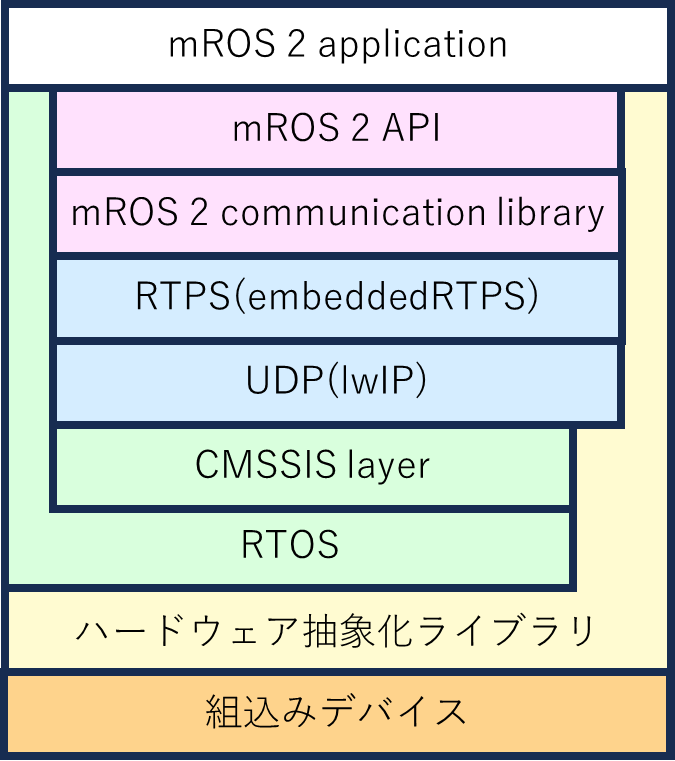
\includegraphics[width=0.9\linewidth]{images/fig1_mros2_b.png}
        \caption{mROS 2の内部構成}
        \label{fig:subfig_b}
    \end{minipage}
\end{figure}

mROS 2は,ROS 2ノードの軽量実行環境である.
このロボットソフトウェア基盤によって,分散型のロボットシステムへの組込み技術の導入ができる.
組込みデバイスは計算資源が限定的であるが,mROS 2を導入することによって組込みデバイスのリアルタイム性の向上および消費電力の削減ができる.
そして,mROS 2がPOSIX[7]に対応したのがmROS 2-POSIXである.
\\ 図1(a)は,mROS 2-POSIXのソフトウェア構成を示す.mROS 2-POSIXアプリケーション層は,ユーザが実装するROS 2ノードに相当する.
mROS 2-POSIX API層および通信ライブラリ層は,メッセージを非同期にパブリッシュやサブスクライブするためのコミュニケーションチャネルであるROS 2のTopicに相当するAPIおよび通信機能を提供する階層である.
本階層は,ROS 2のネイティブなクライアント通信ライブラリであるrclcppと互換性を保つように設計されている.
mROS 2通信ライブラリでは,rclcppのうちpub/sub通信の基本的な機能のみ実装されている.
利用可能な機能は制限されているものの,組込み技術を導入するROS 2開発者は,汎用OS向けのプログラミングスタイルを踏襲しながらC++によってmROS 2のアプリケーションを実装できる.
\\ Real Time Publish-Subscribe(以下,RTPS)プロトコルスタックにはUDPでパブリッシャとサブスクライバC++実装のembeddedRTPS[8]が採用されている.
UDPについては組込み向けのC実装であるlwIPが採用されている.
通信層のembeddedRTPSおよびlwIPはCMSAIS-POSIXに依存しており,図1(b)に示すmROS 2のCMSIS-RTOSを互換した層になっている.
最下層にはハードウェアを抽象化したライブラリがある.
\\ mROS 2-POSIXは図2に示す実行方式を採用している.
リアルタイムOSでは,組込みマイコンを実行資源の管理対象として,タスク単位でアプリケーションが実行される.
POSIXにおいてはタスクに相当する概念はプロセスであり,そこから生成されるスレッドを実行単位として処理が進行している.
しかし,mROS 2-POSIXは実行単位であるノードにPOSIXのスレッドを対応づけ,組込みマイコンでの通信処理におけるイベント割込みについては,POSIX準拠OSにおけるブロッキングAPIの発行に相当させて処理している.

